% ---------------------------------------------------------
% ---- SECTION
% ---------------------------------------------------------
\section{From the continuous Hu-Washizu Lagrangian to the HDG Lagrangian}
\label{sec_appendix_Hu_Washizu}

In this part, the development for the expression of the Hu-Washizu Lagrangian \eqref{eq_0015} is exposed, using the assumptions made in Section \ref{sec_assumtions}.

% ---------------------------------------------------------
% PARAGRAPH
% ---------------------------------------------------------
\paragraph{Element geometry}

In the following, the cell $\cell$ is assumed to be convex.
It is split into a core part $\Bulk \subset \cell$ with boundary $\dBulk$, and into an interface part $\Crown{} \subset \cell$ with boundary $\dCrown = \dBulk \cup \dCell$, as shown in Figure \ref{fig_02}. The interface $\Crown{}$ has some thickness $\ell > 0$ that is supposed to be small compared to $h_{\cell}$ the diameter of $\cell$.

% ---------------------------------------------------------
% PARAGRAPH
% ---------------------------------------------------------
\paragraph{Homothetic transformation}

Let $\tensori{\Xi}{}_{\cell}$ the homothety of ratio $(1 - \alpha \ell)$ and center $\tensori{X}{}_{\cell}$ the centroid of $\cell$, with $0 < \alpha < 1 / \ell$ such that $\Bulk$ (respectively $\dBulk$) is the image of $\cell$ (respectively $\dCell$) by $\tensori{\Xi}{}_{\cell}$. Since $\dBulk$ is an homothety of $\dCell$, any point $\tensori{X}{}_{\dCell} \in \dCell$ and $\tensori{X}{}_{\dBulk} = \tensori{\Xi}{}_{\cell}(\tensori{X}{}_{\dCell}) \in \dBulk$ share the same unit outward normal $\tensori{n}{}$.

% ---------------------------------------------------------
% PARAGRAPH
% ---------------------------------------------------------
\paragraph{Change of reference frame}

Let the change of frame $\tensori{\Psi}$ that takes a point from the reference frame to the local frame with origin on $\dBulk{}$, and whose first direction is given by the normal vector $\tensori{n}$ such that
%
%
%
\begin{equation}
    \begin{aligned}
        \tensori{\Psi} :
        \begin{array}{lll}
            \Crown{} & \rightarrow & \Crown{}
            \\
            \tensori{X} & \mapsto & \tensori{M} = \tensorii{Q}{} \tensori{X} + \tensori{c}
        \end{array}
    \end{aligned}
    % \tensori{\Psi} : \dBulk \rightarrow \dBulk : \tensori{X} \mapsto \tensori{M} = \tensorii{Q}{} \tensori{X} + \tensori{c}
\end{equation}
%
%
%
where $\tensorii{Q}{}$ is the rotation matrix whose first row coincides with $\tensori{n}{}$, and $\tensori{c}$ is a constant vector.

% ---------------------------------------------------------
% PARAGRAPH
% ---------------------------------------------------------
\paragraph{Displacement in the interface}

Assuming that the interface $\Crown$ is thin enough (\textit{i.e.} that $\ell$ is small enough) let assume that the displacement $\tensori{u}{}_{\Crown{}}$ in $\Crown$ linearly bridges $\tensori{u}{}_{\Bulk{}} \vert_{\dBulk{}}$ to $\tensori{u}{}_{\dCell{}}$ such that
%
%
%
\begin{equation}
    \tensori{u}{}_{\Crown{}}(\tensori{M}) =
    \frac{
    \tensori{u}{}_{\dCell{}}(\tensori{\Psi}{}^{-1}(\tensori{M}{}_{\ell}))
    -
    \tensori{u}{}_{\Bulk{}} \vert_{\dBulk{}}(\tensori{\Psi}{}^{-1}(\tensori{M}{}_{o}))
    }
    {\ell}
    M_0
    +
    \tensori{u}{}_{\Bulk{}} \vert_{\dBulk{}}(\tensori{\Psi}{}^{-1}(\tensori{M}{}_{o}))
\end{equation}
%
%
%
where $M_0$ is the first coordinate of a point $\tensori{M}$ in the local frame defined by $\tensori{\Psi}$.
The vector $\tensori{M}{}_{o}$ denotes a point located in the plane $M_0 = 0$, and $\tensori{M}{}_{\ell}$ a point on the plane $M_0 = \ell$, such that they share the same coordinates on their respective planes.
%
% 
% 
\begin{figure}[H]
    \centering
    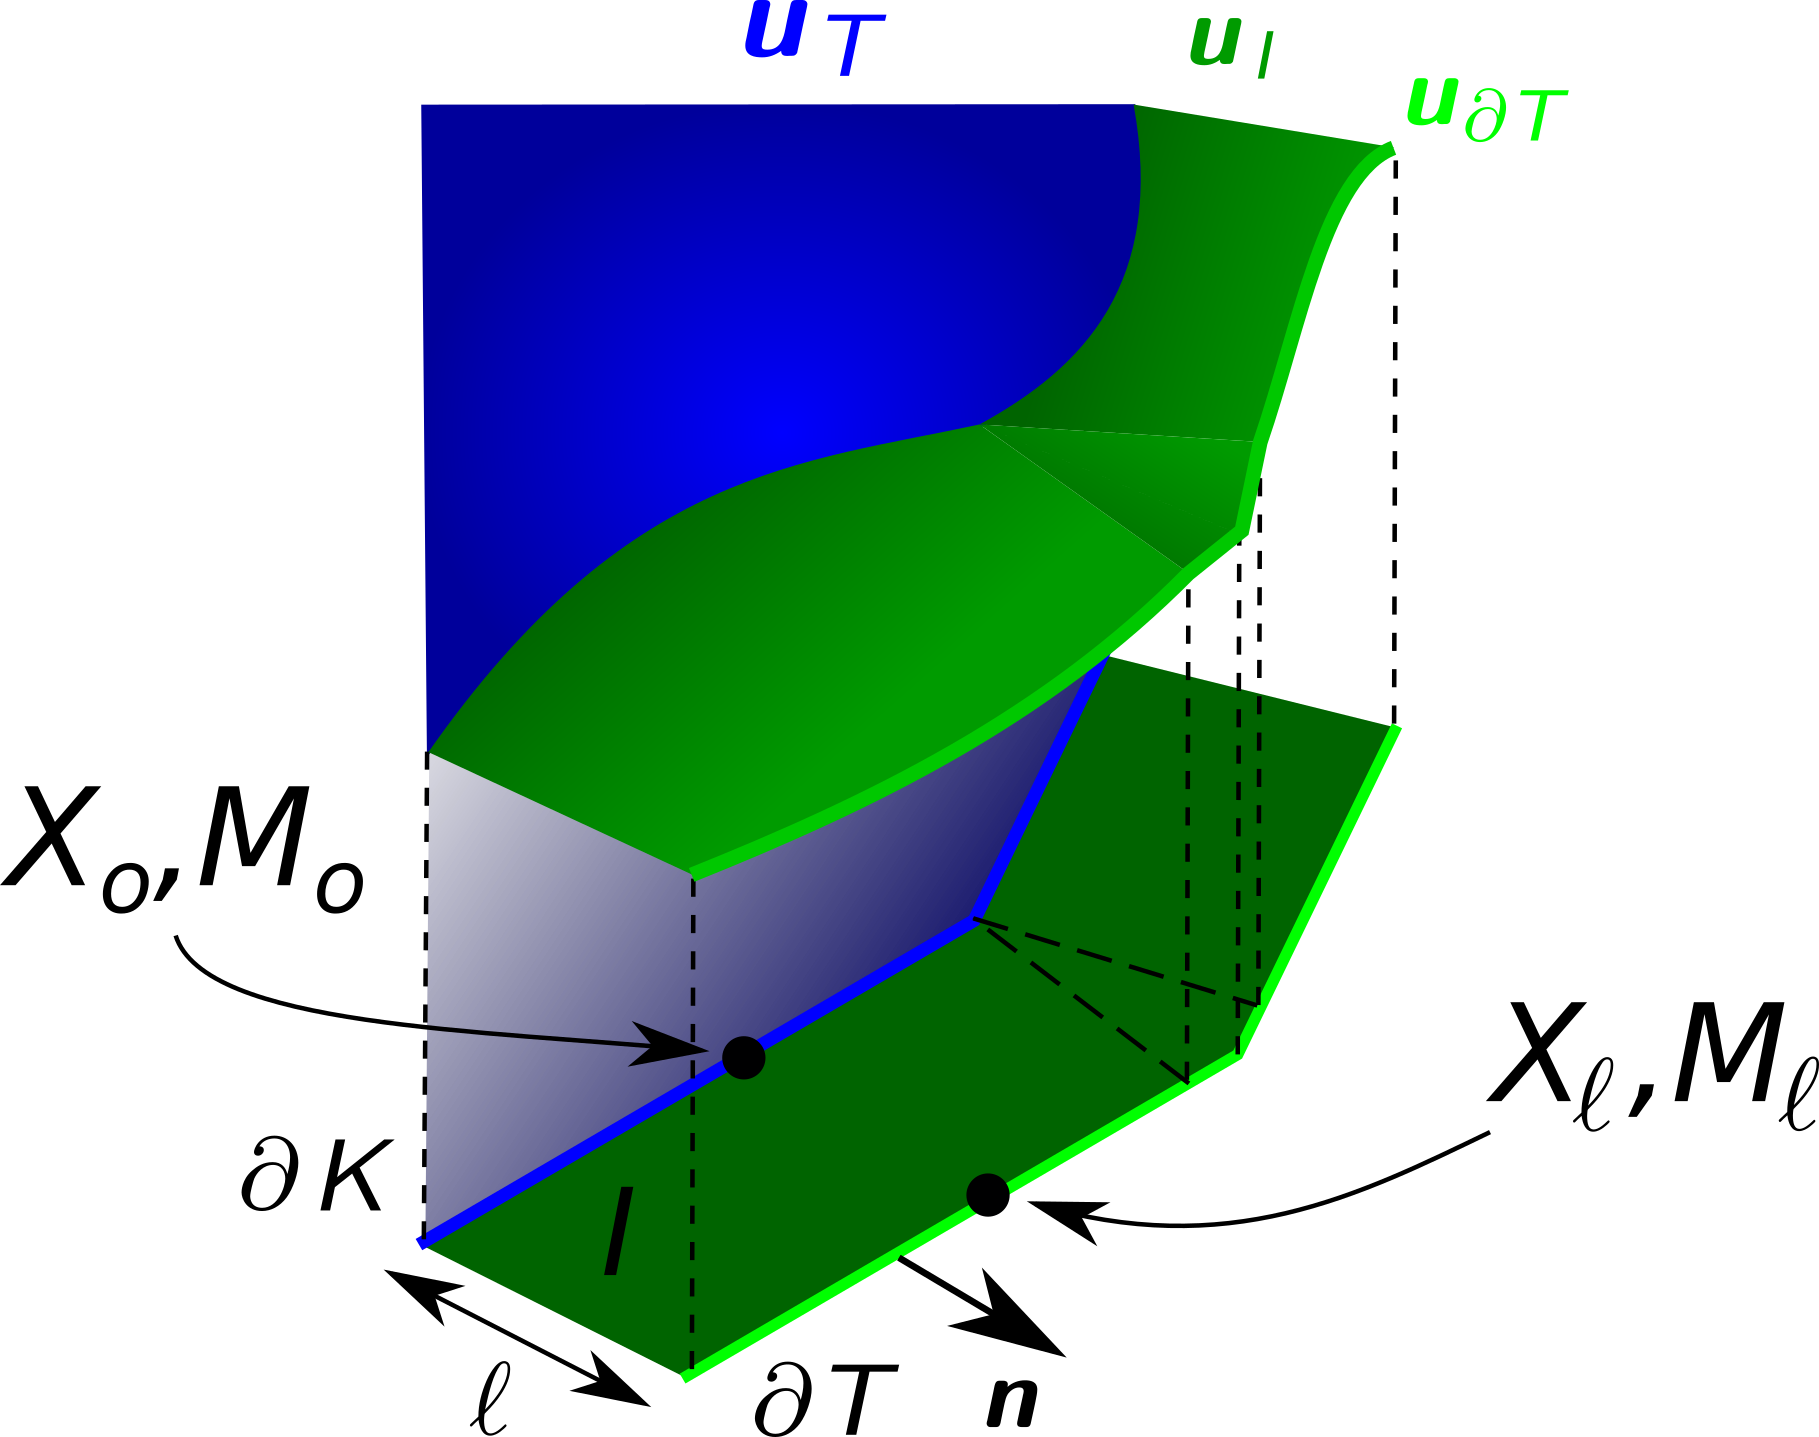
\includegraphics[width=7.cm]{../chapter_002_hho_mechanics/figures/yo.png}
    \caption{schematic representation of the cell, interface and boundary displacement fields close to a corner region}
    \label{fig_appendix_interface_displacement}
\end{figure}
%
%
%
\paragraph{Corners of a cell}

Since corners of the cell meet the intersection of two faces,
the displacement is assumed linear in the interface region around an intersection
such that it linearly bridges the displacement of the cell corner, to that of the two
faces tips (See Figure \ref{fig_appendix_interface_displacement}).
In the following, the corner region is supposed to of the same order of magnitude as $\ell^2$,
such that is is not considered in the following development.

% ---------------------------------------------------------
% PARAGRAPH
% ---------------------------------------------------------
\paragraph{Displacement gradient in the interface}

The derivative of $\tensori{u}{}_{\Crown{}}$ with respect to $\tensori{X}$ yields
%
%
%
\begin{equation}
    \frac{
        \partial \tensoro{u}{}_{\Crown{}i}
    }{
        \partial X_j
    }
    =
    \sum_k
    \frac{
        \partial \tensoro{u}{}_{\Crown{}i}
    }{
        \partial M_k
    }
    \frac{
        \partial M_k
    }{
        \partial X_j
    }
    =
    \frac{
    \tensoro{u}{}_{\dCell{}i}(\tensori{\Psi}{}^{-1}(\tensori{M}{}_{\ell}))
    -
    \tensoro{u}{}_{\Bulk{}i} \vert_{\dBulk{}}(\tensori{\Psi}{}^{-1}(\tensori{M}{}_{o}))
    }
    {\ell}
    Q_{0j}
\end{equation}
%
%
%
which reads
%
%
%
\begin{equation}
    \label{eq_grad_displacement_interface}
    \nabla \tensori{u}{}_{\Crown{}}(\tensori{X}) =
    \frac{
    \tensori{u}{}_{\dCell{}}(\tensori{X}{}_{\ell})
    -
    \tensori{u}{}_{\Bulk{}} \vert_{\dBulk{}}(\tensori{X}{}_{o})
    }
    {\ell}
    \otimes
    \tensori{n}{}
\end{equation}
%
%
%
where the fact that the first row of the rotation matrix $\tensorii{Q}$ is given by $\tensori{n}$ has been used. The points $\tensori{X}{}_{o}$ and $\tensori{X}{}_{\ell}$ are located on the normal plane to $\tensori{n}$ on $\dBulk{}$ and $\dCell{}$ respectively, in the reference frame.

% ---------------------------------------------------------
% PARAGRAPH
% ---------------------------------------------------------
\paragraph{Stress in the interface}

As introduced in Section \ref{sec_appendix_composite_demo}, the stress $\tensorii{P}{}_{\Crown}$ is assumed constant along the direction $\tensori{n}{}$ in $\Crown{}$. By continuity of the traction force across $\dBulk$, the following equality holds true
%
% 
% 
\begin{equation}
    \label{eq_continuity_traction_force_2}
    \begin{aligned}
        (\tensorii{P}{}_{\Crown} - \tensorii{P}{}_{\Bulk} \vert_{\dBulk{}}) \cdot \tensori{n}{} =  0
        &&
        \text{on}
        &&
        \dBulk{}
    \end{aligned}
\end{equation}

% ---------------------------------------------------------
% PARAGRAPH
% ---------------------------------------------------------
\paragraph{Internal Hu-Washizu in the interface}

Let $L_{\Crown{}, \text{int}}^{HW}$ the internal contribution of the Hu-Washizu Lagrangian in $\Crown{}$
%
%
%
\begin{equation}
    \label{eq22}
    \begin{aligned}
        L_{\Crown{}, \text{int}}^{HW}
        := &
        \int_{\Crown{}} \mecPotential{}_{\Crown} + \int_{\Crown{}} (\nabla \tensori{u}{}_{\Crown} - \tensorii{G}{}_{\Crown}) : \tensorii{P}{}_{\Crown}
    \end{aligned}
\end{equation}
%
% 
%
Let $C_\Crown = \{ v \in L^2(\Crown) \ \vert \ v \cdot \tensori{n} = \text{cste} \}$ the set of $L^2$-functions which are constant along the normal axis in $\Crown$. For any function in $C_\Crown$, the following equality holds true:
%
% 
% 
\begin{equation}
    \label{eq_virtual_works0}
        \int_{\Crown} v \ dV
        =
        \int_{\dBulk{}} \int_{\epsilon = 0}^{\ell} v (1 - \alpha \epsilon) \ dS d \epsilon
        =
        \ell (1 - \frac{\alpha}{2} \ell) \int_{\dBulk{}} v \ dS
\end{equation}
%
% 
% 
Noticing that $\nabla \tensori{u}{}_{\Crown} \in C_\Crown$, one has :
%
% 
% 
\begin{equation}
    \begin{aligned}
        \int_{\Crown{}} \mecPotential{}_{\Crown}
        = & 
        \ell (1 - \frac{\alpha}{2} \ell)
        \int_{\dBulk{}} \frac{1}{2} \beta \frac{\ell}{h_{\cell}} \nabla \tensori{u}{}_{\Crown} : \nabla \tensori{u}{}_{\Crown}
        \\
        = & 
        \ell (1 - \frac{\alpha}{2} \ell)
        \int_{\dBulk{}} \frac{\beta}{2 \ell h_{\cell}} (\tensori{u}{}_{\dCell} - \tensori{u}{}_{\Bulk} \vert_{\dBulk}) \otimes
        \tensori{n} : (\tensori{u}{}_{\dCell} - \tensori{u}{}_{\Bulk} \vert_{\dBulk}) \otimes
        \tensori{n}
        \\
        = & 
        \ell (1 - \frac{\alpha}{2} \ell)
        \int_{\dBulk{}} \frac{\beta}{2 \ell h_{\cell}} \lVert \tensori{u}{}_{\dCell} - \tensori{u}{}_{\Bulk}{} \vert_{\dBulk} \lVert {}^2
        \\
        = & 
        (1 - \frac{\alpha}{2} \ell)
        \int_{\dBulk{}} \frac{\beta}{2 h_{\cell}} \lVert \tensori{u}{}_{\dCell} - \tensori{u}{}_{\Bulk}{} \vert_{\dBulk} \lVert {}^2
    \end{aligned}
\end{equation}
%
% 
% 
Moreover, for $\tensorii{P}{}_{\Crown}$ in $C_\Crown{}$ :
%
% 
% 
\begin{equation}
    \begin{aligned}
        \int_{\Crown{}} \nabla \tensori{u}{}_{\Crown} : \tensorii{P}{}_{\Crown}
        = &
        \ell (1 - \frac{\alpha}{2} \ell)
        \int_{\dBulk{}} \nabla \tensori{u}{}_{\Crown} : \tensorii{P}{}_{\Crown}
        \\
        = &
        \ell (1 - \frac{\alpha}{2} \ell)
        \int_{\dBulk{}}
        \frac{1}{\ell}
        (\tensori{u}{}_{\dCell} - \tensori{u}{}_{\Bulk}{} \vert_{\dBulk}) \otimes \tensori{n} : \tensorii{P}{}_{\Crown{}}
        \\
        = &
        (1 - \frac{\alpha}{2} \ell)
        \int_{\dBulk{}}
        (\tensori{u}{}_{\dCell} - \tensori{u}{}_{\Bulk}{} \vert_{\dBulk}) \cdot \tensorii{P}{}_{\Bulk{}} \vert_{\dBulk{}} \cdot \tensori{n}
    \end{aligned}
\end{equation}
% 
% 
% 
where \eqref{eq_continuity_traction_force_2} has been used. And Finally :
%
% 
% 
\begin{equation}
    \begin{aligned}
        L_{\Crown{}, \text{int}}^{HW}
        =
        (1 - \frac{\alpha}{2} \ell)
        \int_{\dBulk{}} \frac{\beta}{2 h_{\cell}} \lVert \tensori{u}{}_{\dCell{}} - \tensori{u}{}_{\Bulk{}} \vert_{\dBulk{}} \rVert^2
        +
        (1 - \frac{\alpha}{2} \ell)
        \int_{\dBulk} (\tensori{u}{}_{\dCell{}} - \tensori{u}{}_{\Bulk{}} \vert_{\dBulk{}}) \cdot \tensorii{P}{}_{\Bulk{}} \vert_{\dBulk{}} \cdot \tensori{n}{}
        -
        \int_{\Crown{}} \tensorii{G}{}_{\Crown{}} : \tensorii{P}{}_{\Crown{}}
    \end{aligned}
\end{equation}

% ---------------------------------------------------------
% PARAGRAPH
% ---------------------------------------------------------
\paragraph{Total Hu-Washizu Lagrangian in the composite element}

Injecting \eqref{eq22} in \eqref{eq_hu_washizu_split} yields
%
% 
% 
\begin{equation}
    \label{eq_0014}
    \begin{aligned}
        L_{\cell}^{HW}
        = &
        \int_{\Bulk} \mecPotential{}_{\bodyLag{}} + (\nabla \tensori{u}{}_{\Bulk} - \tensorii{G}{}_{\Bulk}) : \tensorii{P}{}_{\Bulk}
        % \\
        % &
        +
        (1 - \frac{\alpha}{2} \ell)
        % \Biggl(
        \int_{\dBulk{}} (\tensori{u}{}_{\dCell{}} - \tensori{u}{}_{\Bulk} \vert_{\dBulk}) \cdot \tensorii{P}{}_{\Bulk} \vert_{\dBulk} \cdot \tensori{n}{}
        % \\
        % &
        \\
        &
        +
        (1 - \frac{\alpha}{2} \ell)
        \int_{\dBulk{}} \frac{\beta}{2 h_T} \lVert \tensori{u}{}_{\dCell{}} - \tensori{u}{}_{\Bulk} \vert_{\dBulk{}} \rVert^2
        % \Biggr)
        % \\
        % &
        -
        \int_{\Crown{}} \tensorii{G}{}_{\Crown{}} : \tensorii{P}{}_{\Crown{}}
        % \\
        % &
        -
        \int_{\Bulk} \loadLag \cdot \tensori{u}{}_{\Bulk}
        -
        \int_{\Crown{}} \loadLag \cdot \tensori{u}{}_{\Crown{}}
        -
        \int_{\neumannCell{}} \neumannCellLoad{} \cdot \tensori{u}{}_{\dCell{}}
    \end{aligned}
\end{equation}
%
% 
% 
Since $\ell$ is arbitrary, let $\ell \rightarrow 0$,
the interface region vanishes such that $\Bulk{} \rightarrow \cell$ and $\dBulk{} \rightarrow \dCell$, and the expression of the Hu–Washizu functional over the region $\cell$ writes
% 
% 
%
\begin{equation}
    \label{eq_0015A}
    \begin{aligned}
        L_{\cell}^{HW}
        = &
        \int_{\cell{}} \mecPotential{}_{\bodyLag{}} + (\nabla \tensori{u}{}_{\cell{}} - \tensorii{G}{}_{\cell{}}) : \tensorii{P}{}_{\cell}
        % \\
        % &
        + \int_{\dCell{}} (\tensori{u}{}_{\dCell} - \tensori{u}{}_{\cell} \vert_{\dCell}) \cdot \tensorii{P}{}_{\cell} \vert_{\dCell{}} \cdot \tensori{n}{}
        % \\
        % &
        + \int_{\dCell} \frac{\beta}{2 h_{\cell}} \lVert \tensori{u}{}_{\dCell{}} - \tensori{u}{}_{\cell{}} \vert_{\dCell{}} \rVert^2
        \\
        &
        -
        \int_{\cell} \loadLag{} \cdot \tensori{u}{}_{\cell{}}
        -
        \int_{\neumannCell{}} \neumannCellLoad{} \cdot \tensori{u}{}_{\dCell{}}
    \end{aligned}
\end{equation}
%
%
%
which concludes the development of equation \eqref{eq_0015}.